\documentclass[preprint,12pt,aps,pra,showkeys,amsmath,amssymb,superscriptaddress,floatfix]{revtex4-2}
\usepackage[T1]{fontenc}
\usepackage[utf8]{inputenc}
\usepackage{amsmath,amssymb,amsthm,mathtools,mathrsfs}
\usepackage{microtype,booktabs,enumitem}
\usepackage{xcolor,tikz,etoolbox}
\usepackage[skins,breakable]{tcolorbox}
\usepackage{needspace}
% Keep diagram geometry independent of REVTeX preprint body spacing.
\AtBeginEnvironment{tikzpicture}{\linespread{1}\selectfont}
\usetikzlibrary{arrows.meta,positioning,calc,fit,decorations.pathreplacing}
\usepackage{graphicx}
\usepackage{hyperref}

\definecolor{MMBlue}{RGB}{0,82,155}
\definecolor{MMOrange}{RGB}{200,80,0}
\tikzset{
 mmnode/.style={draw=MMBlue,rounded corners=2pt,fill=MMBlue!4,align=left,execute at begin node={\raggedright},text width=5cm,font=\fontsize{10}{12}\selectfont,inner sep=6pt},
 mmimport/.style={mmnode,draw=black!65,fill=black!4},
 mmcandidate/.style={mmnode,draw=MMOrange,dashed,fill=MMOrange!5},
 mmrejected/.style={mmnode,draw=black,densely dotted,fill=black!8},
 mmproof/.style={->,thick,MMBlue},
 mmflow/.style={->,semithick,black!70},
 mmrepair/.style={->,dashed,thick,MMOrange},
 mmcandidatearrow/.style={->,dashed,semithick,MMOrange},
 mmnote/.style={font=\scriptsize,fill=white,inner sep=2pt,align=center}}

\usepackage[section]{placeins}
\setlength{\emergencystretch}{3em}
\setlist{itemsep=3pt,topsep=4pt}
\newtheorem{theorem}{Theorem}[section]
\newtheorem{proposition}[theorem]{Proposition}
\newtheorem{lemma}[theorem]{Lemma}
\newtheorem{corollary}[theorem]{Corollary}
\theoremstyle{definition}
\newtheorem{definition}[theorem]{Definition}
\newtheorem{example}[theorem]{Example}
\theoremstyle{remark}
\newtheorem{remark}[theorem]{Remark}
% Avoid isolated statement headings and single-line paragraph fragments.
\BeforeBeginEnvironment{theorem}{\Needspace{6\baselineskip}}
\BeforeBeginEnvironment{definition}{\Needspace{5\baselineskip}}
\BeforeBeginEnvironment{proposition}{\Needspace{5\baselineskip}}
\BeforeBeginEnvironment{lemma}{\Needspace{5\baselineskip}}
\BeforeBeginEnvironment{corollary}{\Needspace{5\baselineskip}}
\clubpenalty=5000
\widowpenalty=5000
\newcommand{\R}{\mathbb R}\newcommand{\Z}{\mathbb Z}\newcommand{\N}{\mathbb N}
\newcommand{\Pa}{\operatorname{Pa}}\newcommand{\Desc}{\operatorname{Desc}}
\newcommand{\cl}{\operatorname{cl}}\newcommand{\cost}{\operatorname{cost}}
\newcommand{\status}{\operatorname{status}}
% Faculty cards: a visual rail groups the five faculties within one agent.
% The rail has no arrowhead and does not represent a proof dependency.
\newcommand{\mmfacultybadge}[1]{%
 \node[circle,draw=MMBlue,line width=1pt,fill=white,
 minimum size=7mm,inner sep=0pt,font=\sffamily\small\bfseries,text=MMBlue]
 at ([xshift=15pt,yshift=-15pt]frame.north west) {#1};}
\newcommand{\mmfacultyrail}{%
 \draw[MMBlue!80,line width=1pt]
 ([xshift=15pt,yshift=2pt]frame.north west)--
 ([xshift=15pt,yshift=-2pt]frame.south west);}
\newtcolorbox{mmfacultybox}[2]{enhanced,breakable,
 colback=MMBlue!4,colframe=MMBlue!4,boxrule=0pt,arc=3pt,
 left=39pt,right=9pt,top=4pt,bottom=4pt,
 before skip=2pt,after skip=2pt,
 fontupper=\small\linespread{1.1}\selectfont,
 overlay unbroken={\mmfacultyrail\mmfacultybadge{#1}},
 overlay first={\mmfacultyrail\mmfacultybadge{#1}},
 overlay middle={\mmfacultyrail},overlay last={\mmfacultyrail}}
\newcommand{\mmfaculty}[3]{%
 \begin{mmfacultybox}{#1}{#2}
 {\sffamily\bfseries\color{MMBlue}#2}\par\smallskip #3
 \end{mmfacultybox}}
\newcommand{\agent}[9]{%
 \Needspace{8\baselineskip}
 \subsubsection{#1}
 \noindent\textbf{Object.} #2\par
 \noindent\textbf{Role.} #3\par\smallskip
 \mmfaculty{E}{Ego}{#4}
 \mmfaculty{M}{Memory}{#5}
 \mmfaculty{I}{Intellect}{#6}
 \mmfaculty{S}{Sense}{#7}
 \mmfaculty{A}{Action}{#8}
 \smallskip\noindent #9\par}

\usepackage{longtable,array,calc}
\providecommand{\tightlist}{\setlength{\itemsep}{2pt}\setlength{\parskip}{0pt}}
\makeatletter
\def\frontmatter@abstract@produce{\par\addvspace{\frontmatter@preabstractspace}%
\begingroup\prep@absbox\unvbox\absbox\post@absbox\endgroup
\addvspace{\frontmatter@postabstractspace}}
\makeatother
\newcommand{\field}[2]{\par\smallskip\noindent\textbf{#1.} #2\par}
\setlength{\emergencystretch}{5em}
\AtBeginEnvironment{verbatim}{\small\linespread{1.0}\selectfont}


\hypersetup{colorlinks=true,linkcolor=MMBlue,urlcolor=MMBlue,pdfauthor={Dibakar Sigdel}}

\begin{document}

\title{Banach Fixed-Point Theorem\\[4pt]\large An End-to-End Meta-Math Walkthrough}

\author{Dibakar Sigdel}

\affiliation{Mindverse Computing LLC, Lynnwood, WA 98087, USA}

\date{October 2026}

\begin{abstract}

A complete authored walkthrough of banach fixed-point theorem, with
explicit mathematical contracts, local verification gates, and reusable
exports. The report presents the target theorem, declared imports, a
dependency graph, five-faculty node contracts, a continuous proof, a
worked example, and a hypothesis-repair audit. It is an authored
mathematical exposition, not a deployed-agent transcript or a formal
proof-assistant certificate.

\end{abstract}\maketitle\linespread{1.12}\selectfont

\noindent\textbf{RA-03 / Real Analysis / Report v1}

\section{Target and import contract}

\begin{theorem}

Let \((X,d)\) be a nonempty complete metric space and \(T:X\to X\)
satisfy \(d(Tx,Ty)\le qd(x,y)\) for all \(x,y\), with a fixed
\(0\le q<1\). Then there is a unique \(x_*\) with \(Tx_*=x_*\). From any
\(x_0\in X\), the sequence \(x_{n+1}=Tx_n\) converges to \(x_*\). For
\(0<q<1\),

\[d(x_n,x_*)\le\frac{q^n}{1-q}d(x_1,x_0).\]

The output is an existence proof, a uniqueness proof, a convergent
construction, and an error certificate. An iterate with small
consecutive displacement is an approximation; it is not automatically an
exact fixed point.

\end{theorem}

\subsection{Foundations and permitted imports}

completeness means every Cauchy sequence in X has a limit in X; a
contraction has one uniform factor q; geometric-series summation and the
triangle inequality are imported. If \(q=0\), T is constant, so \(x_1\)
is already a fixed point. We prove the remaining case \(0<q<1\).

\clearpage\section{Node interaction workflow}

\begin{center}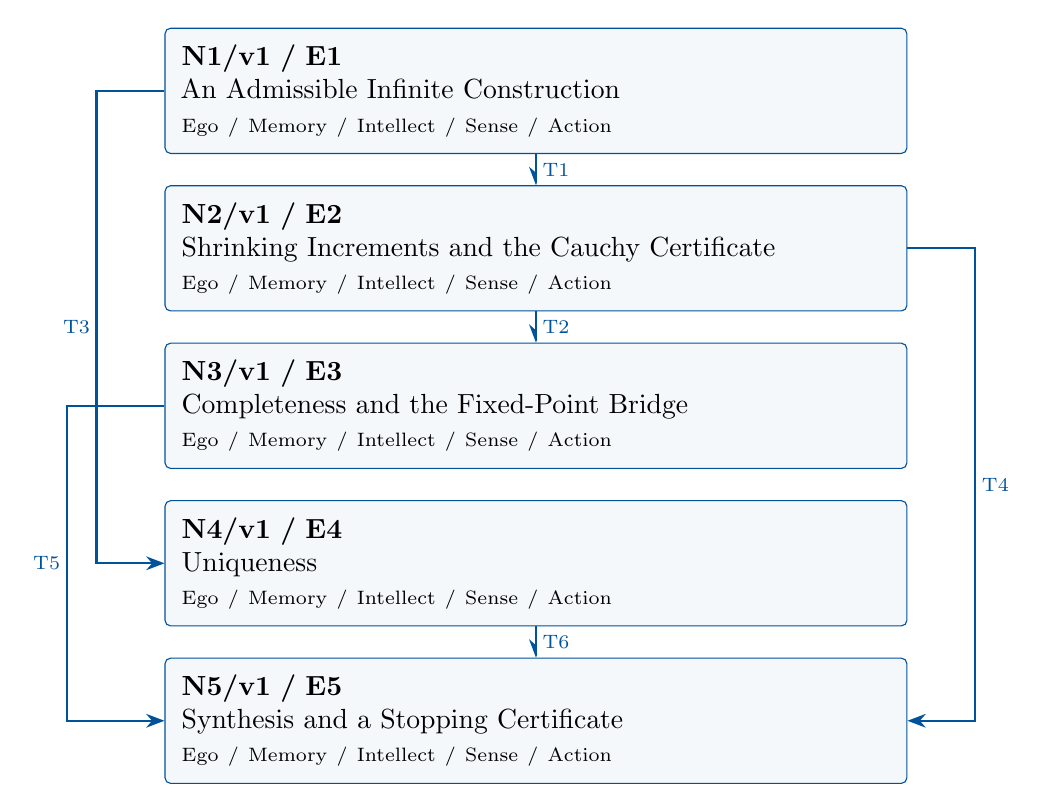
\begin{tikzpicture}[>=Stealth,x=1cm,y=1cm]

\node[mmnode,text width=9cm,minimum height=1.25cm] (N1) at (0,0.0) {\textbf{N1/v1 / E1}\\An Admissible Infinite Construction\\{\scriptsize Ego / Memory / Intellect / Sense / Action}};

\node[mmnode,text width=9cm,minimum height=1.25cm] (N2) at (0,-2.0) {\textbf{N2/v1 / E2}\\Shrinking Increments and the Cauchy Certificate\\{\scriptsize Ego / Memory / Intellect / Sense / Action}};

\node[mmnode,text width=9cm,minimum height=1.25cm] (N3) at (0,-4.0) {\textbf{N3/v1 / E3}\\Completeness and the Fixed-Point Bridge\\{\scriptsize Ego / Memory / Intellect / Sense / Action}};

\node[mmnode,text width=9cm,minimum height=1.25cm] (N4) at (0,-6.0) {\textbf{N4/v1 / E4}\\Uniqueness\\{\scriptsize Ego / Memory / Intellect / Sense / Action}};

\node[mmnode,text width=9cm,minimum height=1.25cm] (N5) at (0,-8.0) {\textbf{N5/v1 / E5}\\Synthesis and a Stopping Certificate\\{\scriptsize Ego / Memory / Intellect / Sense / Action}};

\draw[mmproof] (N1.south) -- node[mmnote,right] {T1} (N2.north);

\draw[mmproof] (N2.south) -- node[mmnote,right] {T2} (N3.north);

\draw[mmproof] (N1.west) -- (-5.58,0) -- node[mmnote,left] {T3} (-5.58,-6) -- (N4.west);

\draw[mmproof] (N2.east) -- (5.58,-2) -- node[mmnote,right] {T4} (5.58,-8) -- (N5.east);

\draw[mmproof] (N3.west) -- (-5.96,-4) -- node[mmnote,left] {T5} (-5.96,-8) -- (N5.west);

\draw[mmproof] (N4.south) -- node[mmnote,right] {T6} (N5.north);

\end{tikzpicture}\end{center}

Each box is one mathematical agent containing all five faculties. Blue
arrows carry the versioned exports listed below. The layout gives a
reading order; only drawn arrows assert dependencies. Diagnostic repair
is separate from the proof DAG.

\clearpage\subsection{Versioned evidence-transfer ledger}

\begingroup\small\linespread{1.05}\selectfont

\Needspace{5\baselineskip}\field{T1: N1/E1/v1 to N2}{For every \(x_0\in X\), \(x_{n+1}=T(x_n)\) stays in the nonempty
complete space \(X\).}

\field{Receiving activity}{N2: Shrinking Increments and the Cauchy Certificate}

\field{Compatibility}{Use the same mathematical objects and hypotheses as the source export.
Receiving contract: N1/E1 and the finite geometric-series bound.}

\Needspace{5\baselineskip}\field{T2: N2/E2/v1 to N3}{\(d(x_{n+p},x_n)\le q^n d(x_1,x_0)/(1-q)\); the iterates are Cauchy.}

\field{Receiving activity}{N3: Completeness and the Fixed-Point Bridge}

\field{Compatibility}{Use the same mathematical objects and hypotheses as the source export.
Receiving contract: N2/E2 and completeness of the original metric space.}

\Needspace{5\baselineskip}\field{T3: N1/E1/v1 to N4}{For every \(x_0\in X\), \(x_{n+1}=T(x_n)\) stays in the nonempty
complete space \(X\).}

\field{Receiving activity}{N4: Uniqueness}

\field{Compatibility}{Use the same mathematical objects and hypotheses as the source export.
Receiving contract: N1/E1; two putative exact fixed points \(u,v\).}

\Needspace{5\baselineskip}\field{T4: N2/E2/v1 to N5}{\(d(x_{n+p},x_n)\le q^n d(x_1,x_0)/(1-q)\); the iterates are Cauchy.}

\field{Receiving activity}{N5: Synthesis and a Stopping Certificate}

\field{Compatibility}{Use the same mathematical objects and hypotheses as the source export.
Receiving contract: N2/E2, N3/E3, and N4/E4.}

\Needspace{5\baselineskip}\field{T5: N3/E3/v1 to N5}{There exists \(x_*\in X\) with \(T(x_*)=x_*\) and
\(d(x_n,x_*)\le q^n d(x_1,x_0)/(1-q)\).}

\field{Receiving activity}{N5: Synthesis and a Stopping Certificate}

\field{Compatibility}{Use the same mathematical objects and hypotheses as the source export.
Receiving contract: N2/E2, N3/E3, and N4/E4.}

\Needspace{5\baselineskip}\field{T6: N4/E4/v1 to N5}{Any two fixed points in \(X\) are equal.}

\field{Receiving activity}{N5: Synthesis and a Stopping Certificate}

\field{Compatibility}{Use the same mathematical objects and hypotheses as the source export.
Receiving contract: N2/E2, N3/E3, and N4/E4.}

\endgroup

\clearpage\section{Agent roles and five-faculty activities}\begingroup\small\linespread{1.05}\selectfont\setlist{itemsep=1pt,topsep=2pt}

\subsection{N1/v1: An Admissible Infinite Construction}

\field{Object and role}{An Admissible Infinite Construction. Establish the following local
result: For every \(x_0\in X\), \(x_{n+1}=T(x_n)\) stays in the nonempty
complete space \(X\).}

\field{Inputs}{\(T:X\to X\) and a uniform contraction constant \(0\le q<1\).}

\mmfaculty{E}{Ego}{Own E1/v1: For every \(x_0\in X\), \(x_{n+1}=T(x_n)\) stays in the
nonempty complete space \(X\).}

\mmfaculty{M}{Memory}{Metric and map definitions}

\mmfaculty{I}{Intellect}{Choose any starting point}

\mmfaculty{S}{Sense}{Check completeness, self-map, \(q<1\)}

\mmfaculty{A}{Action}{Carry out the numbered deductions and publish E1/v1 together with its
hypotheses and proof location.}

\smallskip\noindent\textbf{Numbered mathematical activities}

\begin{enumerate}[label=N1.\arabic*,leftmargin=3.4em]

\item Check nonemptiness, completeness, the self-map condition, and a single
global constant \(q\).

\item If \(q=0\), the map is constant and its value is its unique fixed point.

\item For \(0<q<1\), fix any \(x_0\) and form the iteration.

\end{enumerate}

\field{Export E1/v1}{For every \(x_0\in X\), \(x_{n+1}=T(x_n)\) stays in the nonempty
complete space \(X\).}

\field{Acceptance gate}{Check completeness, self-map, \(q<1\) Publish only after checking every
displayed deduction.}

\field{Targeted repair}{If the check fails, revise N1: Check completeness, self-map, \(q<1\)
Recheck dependent nodes N2, N3, N4, N5.}

\clearpage

\subsection{N2/v1: Shrinking Increments and the Cauchy Certificate}

\field{Object and role}{Shrinking Increments and the Cauchy Certificate. Establish the following
local result: \(d(x_{n+p},x_n)\le q^n d(x_1,x_0)/(1-q)\); the iterates
are Cauchy.}

\field{Inputs}{N1/E1 and the finite geometric-series bound.}

\mmfaculty{E}{Ego}{Own E2/v1: \(d(x_{n+p},x_n)\le q^n d(x_1,x_0)/(1-q)\); the iterates are
Cauchy.}

\mmfaculty{M}{Memory}{Geometric series}

\mmfaculty{I}{Intellect}{Sum shrinking increments}

\mmfaculty{S}{Sense}{Keep q uniform}

\mmfaculty{A}{Action}{Carry out the numbered deductions and publish E2/v1 together with its
hypotheses and proof location.}

\smallskip\noindent\textbf{Numbered mathematical activities}

\begin{enumerate}[label=N2.\arabic*,leftmargin=3.4em]

\item Inductively prove \(d(x_{n+1},x_n)\le q^n d(x_1,x_0)\).

\item Sum increments from \(n\) to \(n+p\) using the triangle inequality.

\item Let \(n\) grow while keeping the tail estimate uniform in \(p\).

\end{enumerate}

\field{Export E2/v1}{\(d(x_{n+p},x_n)\le q^n d(x_1,x_0)/(1-q)\); the iterates are Cauchy.}

\field{Acceptance gate}{Keep q uniform Publish only after checking every displayed deduction.}

\field{Targeted repair}{If the check fails, revise N2: Keep q uniform Recheck dependent nodes
N3, N5.}

\clearpage

\subsection{N3/v1: Completeness and the Fixed-Point Bridge}

\field{Object and role}{Completeness and the Fixed-Point Bridge. Establish the following local
result: There exists \(x_*\in X\) with \(T(x_*)=x_*\) and
\(d(x_n,x_*)\le q^n d(x_1,x_0)/(1-q)\).}

\field{Inputs}{N2/E2 and completeness of the original metric space.}

\mmfaculty{E}{Ego}{Own E3/v1: There exists \(x_*\in X\) with \(T(x_*)=x_*\) and
\(d(x_n,x_*)\le q^n d(x_1,x_0)/(1-q)\).}

\mmfaculty{M}{Memory}{Completeness}

\mmfaculty{I}{Intellect}{Use contraction continuity}

\mmfaculty{S}{Sense}{Keep limit in X}

\mmfaculty{A}{Action}{Carry out the numbered deductions and publish E3/v1 together with its
hypotheses and proof location.}

\smallskip\noindent\textbf{Numbered mathematical activities}

\begin{enumerate}[label=N3.\arabic*,leftmargin=3.4em]

\item Take the Cauchy limit inside \(X\).

\item Use \(d(Tx_*,x_*)\le qd(x_*,x_n)+d(x_{n+1},x_*)\) and pass to the limit.

\item Let the tail endpoint tend to infinity in the estimate.

\end{enumerate}

\field{Export E3/v1}{There exists \(x_*\in X\) with \(T(x_*)=x_*\) and
\(d(x_n,x_*)\le q^n d(x_1,x_0)/(1-q)\).}

\field{Acceptance gate}{Keep limit in X Publish only after checking every displayed deduction.}

\field{Targeted repair}{If the check fails, revise N3: Keep limit in X Recheck dependent nodes
N5.}

\clearpage

\subsection{N4/v1: Uniqueness}

\field{Object and role}{Uniqueness. Establish the following local result: Any two fixed points
in \(X\) are equal.}

\field{Inputs}{N1/E1; two putative exact fixed points \(u,v\).}

\mmfaculty{E}{Ego}{Own E4/v1: Any two fixed points in \(X\) are equal.}

\mmfaculty{M}{Memory}{Distance axioms}

\mmfaculty{I}{Intellect}{Apply contraction to their distance}

\mmfaculty{S}{Sense}{Compare exact fixed points}

\mmfaculty{A}{Action}{Carry out the numbered deductions and publish E4/v1 together with its
hypotheses and proof location.}

\smallskip\noindent\textbf{Numbered mathematical activities}

\begin{enumerate}[label=N4.\arabic*,leftmargin=3.4em]

\item Apply the contraction inequality to \(u,v\).

\item Obtain \((1-q)d(u,v)\le0\).

\item Use \(1-q>0\) and the metric separation axiom.

\end{enumerate}

\field{Export E4/v1}{Any two fixed points in \(X\) are equal.}

\field{Acceptance gate}{Compare exact fixed points Publish only after checking every displayed
deduction.}

\field{Targeted repair}{If the check fails, revise N4: Compare exact fixed points Recheck
dependent nodes N5.}

\clearpage

\subsection{N5/v1: Synthesis and a Stopping Certificate}

\field{Object and role}{Synthesis and a Stopping Certificate. Establish the following local
result: The unique fixed point is reached in the limit from every
starting point, with \(d(x_n,x_*)\le d(x_n,x_{n+1})/(1-q)\).}

\field{Inputs}{N2/E2, N3/E3, and N4/E4.}

\mmfaculty{E}{Ego}{Own E5/v1: The unique fixed point is reached in the limit from every
starting point, with \(d(x_n,x_*)\le d(x_n,x_{n+1})/(1-q)\).}

\mmfaculty{M}{Memory}{All predecessor certificates}

\mmfaculty{I}{Intellect}{Join construction and bounds}

\mmfaculty{S}{Sense}{Separate approximation from equality}

\mmfaculty{A}{Action}{Carry out the numbered deductions and publish E5/v1 together with its
hypotheses and proof location.}

\smallskip\noindent\textbf{Numbered mathematical activities}

\begin{enumerate}[label=N5.\arabic*,leftmargin=3.4em]

\item Restart the geometric-tail estimate at index \(n\).

\item Use the observed next increment to produce a certified stopping
tolerance.

\item Combine existence, uniqueness, and both error estimates without equating
a finite iterate to the exact limit.

\end{enumerate}

\field{Export E5/v1}{The unique fixed point is reached in the limit from every starting
point, with \(d(x_n,x_*)\le d(x_n,x_{n+1})/(1-q)\).}

\field{Acceptance gate}{Separate approximation from equality Publish only after checking every
displayed deduction.}

\field{Targeted repair}{If the check fails, revise N5: Separate approximation from equality
Withhold this terminal result until its gate passes.}

\endgroup\clearpage\section{Continuous mathematical proof}\label{sec:proof}

\subsection{N1 --- An Admissible Infinite
Construction}\label{n1-an-admissible-infinite-construction}

Choose \(x_0\in X\) and put \(x_{n+1}=Tx_n\). Every iterate stays in X
because T is a self-map. Set \(D=d(x_1,x_0)\). If \(D=0\), the initial
point is already fixed. Otherwise the following estimates still apply
without changing the algorithm.

\subsection{N2 --- Shrinking Increments and the Cauchy
Certificate}\label{n2-shrinking-increments-and-the-cauchy-certificate}

Induction using the contraction gives

\[d(x_{n+1},x_n)\le q^nD.\]

For \(m>n\), the triangle inequality therefore gives

\[d(x_m,x_n)\le\sum_{k=n}^{m-1}q^kD\le\frac{q^nD}{1-q}.\]

The bound tends to zero independently of m. Given any epsilon, choose n
large enough that the last expression is smaller than epsilon. Thus the
sequence is Cauchy. This is a statement about every sufficiently late
pair of iterates, not just adjacent ones.

\subsection{N3 --- Completeness and the Fixed-Point
Bridge}\label{n3-completeness-and-the-fixed-point-bridge}

Completeness supplies \(x_*\in X\) with \(x_n\to x_*\). Since

\[d(Tx_*,x_*)\le d(Tx_*,Tx_n)+d(x_{n+1},x_*)\le qd(x_*,x_n)+d(x_{n+1},x_*),\]

the right side tends to zero. Hence \(Tx_*=x_*\). Letting m tend to
infinity in N2's estimate gives the stated error bound. The continuity
used here follows from the contraction inequality itself.

\subsection{N4 --- Uniqueness}\label{n4-uniqueness}

If x and y are fixed points, then \(d(x,y)=d(Tx,Ty)\le qd(x,y)\).
Consequently \((1-q)d(x,y)\le0\). As \(1-q>0\) and distance is
nonnegative, \(d(x,y)=0\), so \(x=y\).

\subsection{N5 --- Synthesis and a Stopping
Certificate}\label{n5-synthesis-and-a-stopping-certificate}

Every initial point has a limit by N2--N3, and N4 shows all those limits
are the same point. For a practical stopping criterion, N2 applied
starting at \(x_n\) gives

\[d(x_n,x_*)\le\frac{d(x_{n+1},x_n)}{1-q}.\]

For \(n\ge 1\) there is also the sharper bound

\[d(x_n,x_*)\le\frac{q}{1-q}d(x_n,x_{n-1}).\]

Thus a requested tolerance can be met using observed increments and a
proved contraction factor. This completes the theorem. \(\square\)

\hfill$\square$

\section{Worked orchestration}

Take \(X=[0,1]\) with ordinary distance and \(T(x)=\operatorname{cos}\)
x. The interval is complete, and T maps it into {[}cos 1,1{]}, a subset
of X. The mean value theorem gives \(|\cos x-\cos y|\le(\sin1)|x-y|\).
Use \(q=\sin1\approx0.841471<1\).

Starting from \(x_0=0\):

\begin{itemize}
\item
  \textbf{n}

  0

  \textbf{Approximate iterate}

  0
\item
  \textbf{n}

  1

  \textbf{Approximate iterate}

  1
\item
  \textbf{n}

  2

  \textbf{Approximate iterate}

  0.540302306
\item
  \textbf{n}

  3

  \textbf{Approximate iterate}

  0.857553216
\item
  \textbf{n}

  4

  \textbf{Approximate iterate}

  0.654289790
\item
  \textbf{n}

  5

  \textbf{Approximate iterate}

  0.793480359
\end{itemize}

The alternation does not invalidate convergence. A contraction bound
controls its shrinking oscillations. After 100 iterations, the a priori
error bound is \(q^{100}/(1-q)<2.1\times10^{-7}\). The limit is
approximately 0.7390851332; this decimal is illustrative, while the
theorem establishes the unique exact solution in {[}0,1{]}.

\subsection{Boundary and hypothesis audit}

\begin{itemize}
\item
  \textbf{Boundary}

  \(q=0\)

  \textbf{Consequence}

  T is constant; one application reaches the fixed point
\item
  \textbf{Boundary}

  \(q=1\)

  \textbf{Consequence}

  Identity on a multi-point space has many fixed points; uniqueness
  fails
\item
  \textbf{Boundary}

  Missing completeness

  \textbf{Consequence}

  Limit may leave the space
\item
  \textbf{Boundary}

  Map leaves X

  \textbf{Consequence}

  Iteration is not covered by the contract
\item
  \textbf{Boundary}

  Finite decimal equality

  \textbf{Consequence}

  Does not certify an exact fixed point
\end{itemize}

Export the contraction theorem, uniqueness lemma, and both error
estimates with their hypotheses. The
\href{../../../2-Analysis/Advanced-Calculus/projects/inverse-function-theorem.md}{Inverse
Function Theorem example} imports this completed module to solve nearby
equations.

\section{Illustrative failure and repair}

The following is an authored diagnostic scenario. Changed assumptions
define a new contract; they do not retroactively prove the original
statement.

\subsection{Failure and correction}
Consider \(T(x)=x/2\) on \(X=(0,1)\). A proposed branch claims a fixed
point because the distances halve. Sense finds that X is not complete:
the iterates converge to 0, which is missing.

\begin{itemize}
\item
  \textbf{Node:} N3
\item
  \textbf{State:} STALLED
\item
  \textbf{Failing faculty:} Sense
\item
  \textbf{Failed hypothesis:} complete domain containing the limit
\item
  \textbf{Example:} \(T(x)=x/2\) on (0,1)
\item
  \textbf{Repair target:} N1
\item
  \textbf{Blocked export:} fixed-point existence in (0,1)
\end{itemize}

Memory retrieves completeness's definition. Sense retains the
missing-point diagnosis. Intellect proposes {[}0,1{]} for this example.
Action verifies that the repaired domain is complete and invariant and
that 0 is fixed. Ego publishes a theorem for the repaired domain while
recording that the original map on (0,1) has no fixed point. Repair does
not retroactively prove the rejected original claim.

\subsection{Hypothesis boundary}
\begin{itemize}
\item
  \textbf{Boundary}

  \(q=0\)

  \textbf{Consequence}

  T is constant; one application reaches the fixed point
\item
  \textbf{Boundary}

  \(q=1\)

  \textbf{Consequence}

  Identity on a multi-point space has many fixed points; uniqueness
  fails
\item
  \textbf{Boundary}

  Missing completeness

  \textbf{Consequence}

  Limit may leave the space
\item
  \textbf{Boundary}

  Map leaves X

  \textbf{Consequence}

  Iteration is not covered by the contract
\item
  \textbf{Boundary}

  Finite decimal equality

  \textbf{Consequence}

  Does not certify an exact fixed point
\end{itemize}

Export the contraction theorem, uniqueness lemma, and both error
estimates with their hypotheses. The
\href{../../../2-Analysis/Advanced-Calculus/projects/inverse-function-theorem.md}{Inverse
Function Theorem example} imports this completed module to solve nearby
equations.

\subsection{Version and recheck}
Treat any changed assumption as a new contract. Recheck the revised
export and all of its descendants. A backward diagnostic never
establishes an earlier theorem. This is an authored teaching trace, not
an execution log.

\par\medskip\begingroup\small\linespread{1.0}\selectfont\noindent\textbf{Provenance.} This authored proof is complete relative to its declared imports. Reuse
each export with its assumptions, proof, and version. The original
Markdown remains available for comparison.
\par\endgroup

\par\smallskip\begingroup\small\linespread{1.0}\selectfont\noindent\textbf{Further reading.} \href{https://www2.math.upenn.edu/~gressman/analysis/12-inversefuncthm.html}{University
of Pennsylvania advanced-analysis material on contraction-based
inversion}.\par\endgroup

\end{document}
